\subsubsection{\stid{4.08} ExaHDF5}\label{subsubsect:exahdf5}

\paragraph{Overview} 


Hierarchical Data Format version 5 (HDF5) is the most popular high-level I/O library for scientific applications to write and read data files. The HDF Group released the first version of HDF5 in 1998 and over the past 20 years, it has been used by numerous applications not only in scientific domains but also in finance, space technologies, etc. HDF5 is the most used library for performing parallel I/O on existing HPC systems at the DOE supercomputing facilities. NASA gives HDF5 software the highest technology readiness level (TRL 9), which is given to actual systems “flight proven” through successful mission operations.

In this project, various HDF5 features are in development to address efficiency and other challenges posed by data management and parallel I/O on exascale architectures. The ExaHDF5 team is productizing features and techniques that have been previously prototyped, exploring optimization strategies on upcoming architectures, maintaining and optimizing existing HDF5 features tailored for ECP applications. Along with supporting and optimizing I/O performance of HDF5 applications, new features in this project include transparent data caching in the multi-level storage hierarchy, topology-aware I/O related data movement in exascale systems, full single-writer and multi-reader (SWMR) for workflows, asynchronous I/O, data and metadata querying. 

Many of the funded exascale applications and co-design centers require HDF5 for their I/O, and enhancing the HDF5 software to handle the unique challenges of exascale architectures will play an instrumental role in the success of the ECP. For instance, AMReX, the AMR co-design center is using HDF5 for I/O, and all the ECP applications that are collaborating with AMReX will benefit from HDF5. Full SWMR feature will support the needs of ExaFEL’s workflow in appending data incrementally. Virtual Object Layer (VOL) and interoperability features with netCDF and ADIOS data opens up the rich HDF5 data management interface to a large number of file formats. The project will be releasing these new features in HDF5 for broad deployment on HPC systems. Focusing on the challenges of exascale I/O, technologies will be developed based on the massively parallel storage hierarchies that are being built into pre-exascale systems. The enhanced HDF5 software will achieve efficient parallel I/O on exascale systems in ways that will impact a large number of DOE science as well as industrial applications.

\paragraph{Key  Challenges}
\paragraph{}
There are challenges in developing I/O strategies for using a hierarchy of storage devices and topology of compute nodes efficiently, developing interoperability features with other file formats, and integrating existing prototyped features into production releases. 

\textit{Efficient use of hierarchical storage and topology.} Data generation (e.g. by simulations) and consumption (such as for analysis) in exascale applications may span various storage and memory tiers, including near-memory NVRAM, SSD-based burst buffers, fast disk, campaign storage, and archival storage. Effective support for caching and prefetching data based on the needs of the application is critical for scalable performance. Also, support for higher bandwidth transfers and lower message latency interconnects in supercomputers are becoming more complex, in terms of both topology as well as routing policies. I/O libraries need to fully account for this topology in order to
maximize I/O performance, and current I/O mechanisms fail to exploit the system topology efficiently.

\textit{Interoperability with other file formats.} HDF5 offers a rich data model and strong features for accessing data, and using these capabilities to access data stored in other data formats would be a valuable productivity boost to applications. The team is developing to add interoperability features that will enable ECP applications to use HDF5 function calls to read from other file formats directly. Development includes functionality to read “classic” netCDF (including PnetCDF) and ADIOS/BP files, as these formats are in active use in DOE application communities focused on exascale deliverables. 

\paragraph{Solution Strategy}

\textit{Utilizing complex compute and storage hardware. } To use multi-level storage hierarchy, Data Elevator is being developed in this project. The Data Elevator library intercepts HDF5 file open calls and redirects them to intermediate and faster caching storage layers, where application reads or writes data. When updates or writes to the intermediate data is done, a server daemon of the Data Elevator moves the data transparently to its final destination on colder storage layers, such as disk-based parallel file system, without modifying the source code or placing the burden on user to move the data explicitly from the intermediate storage layer.

In our prior work, improved communication times were achieved for a wide spectrum of data movement patterns such as those seen in multi-physics codes, parallel I/O aggregation, and in situ analysis, and have also improved the time to access parallel file systems. The team is developing these topology-aware optimization strategies as a Virtual File Driver (VFD), which can be plugged in to HDF5. 

\begin{wrapfigure}{r}{0.5\textwidth}
  \begin{center}
    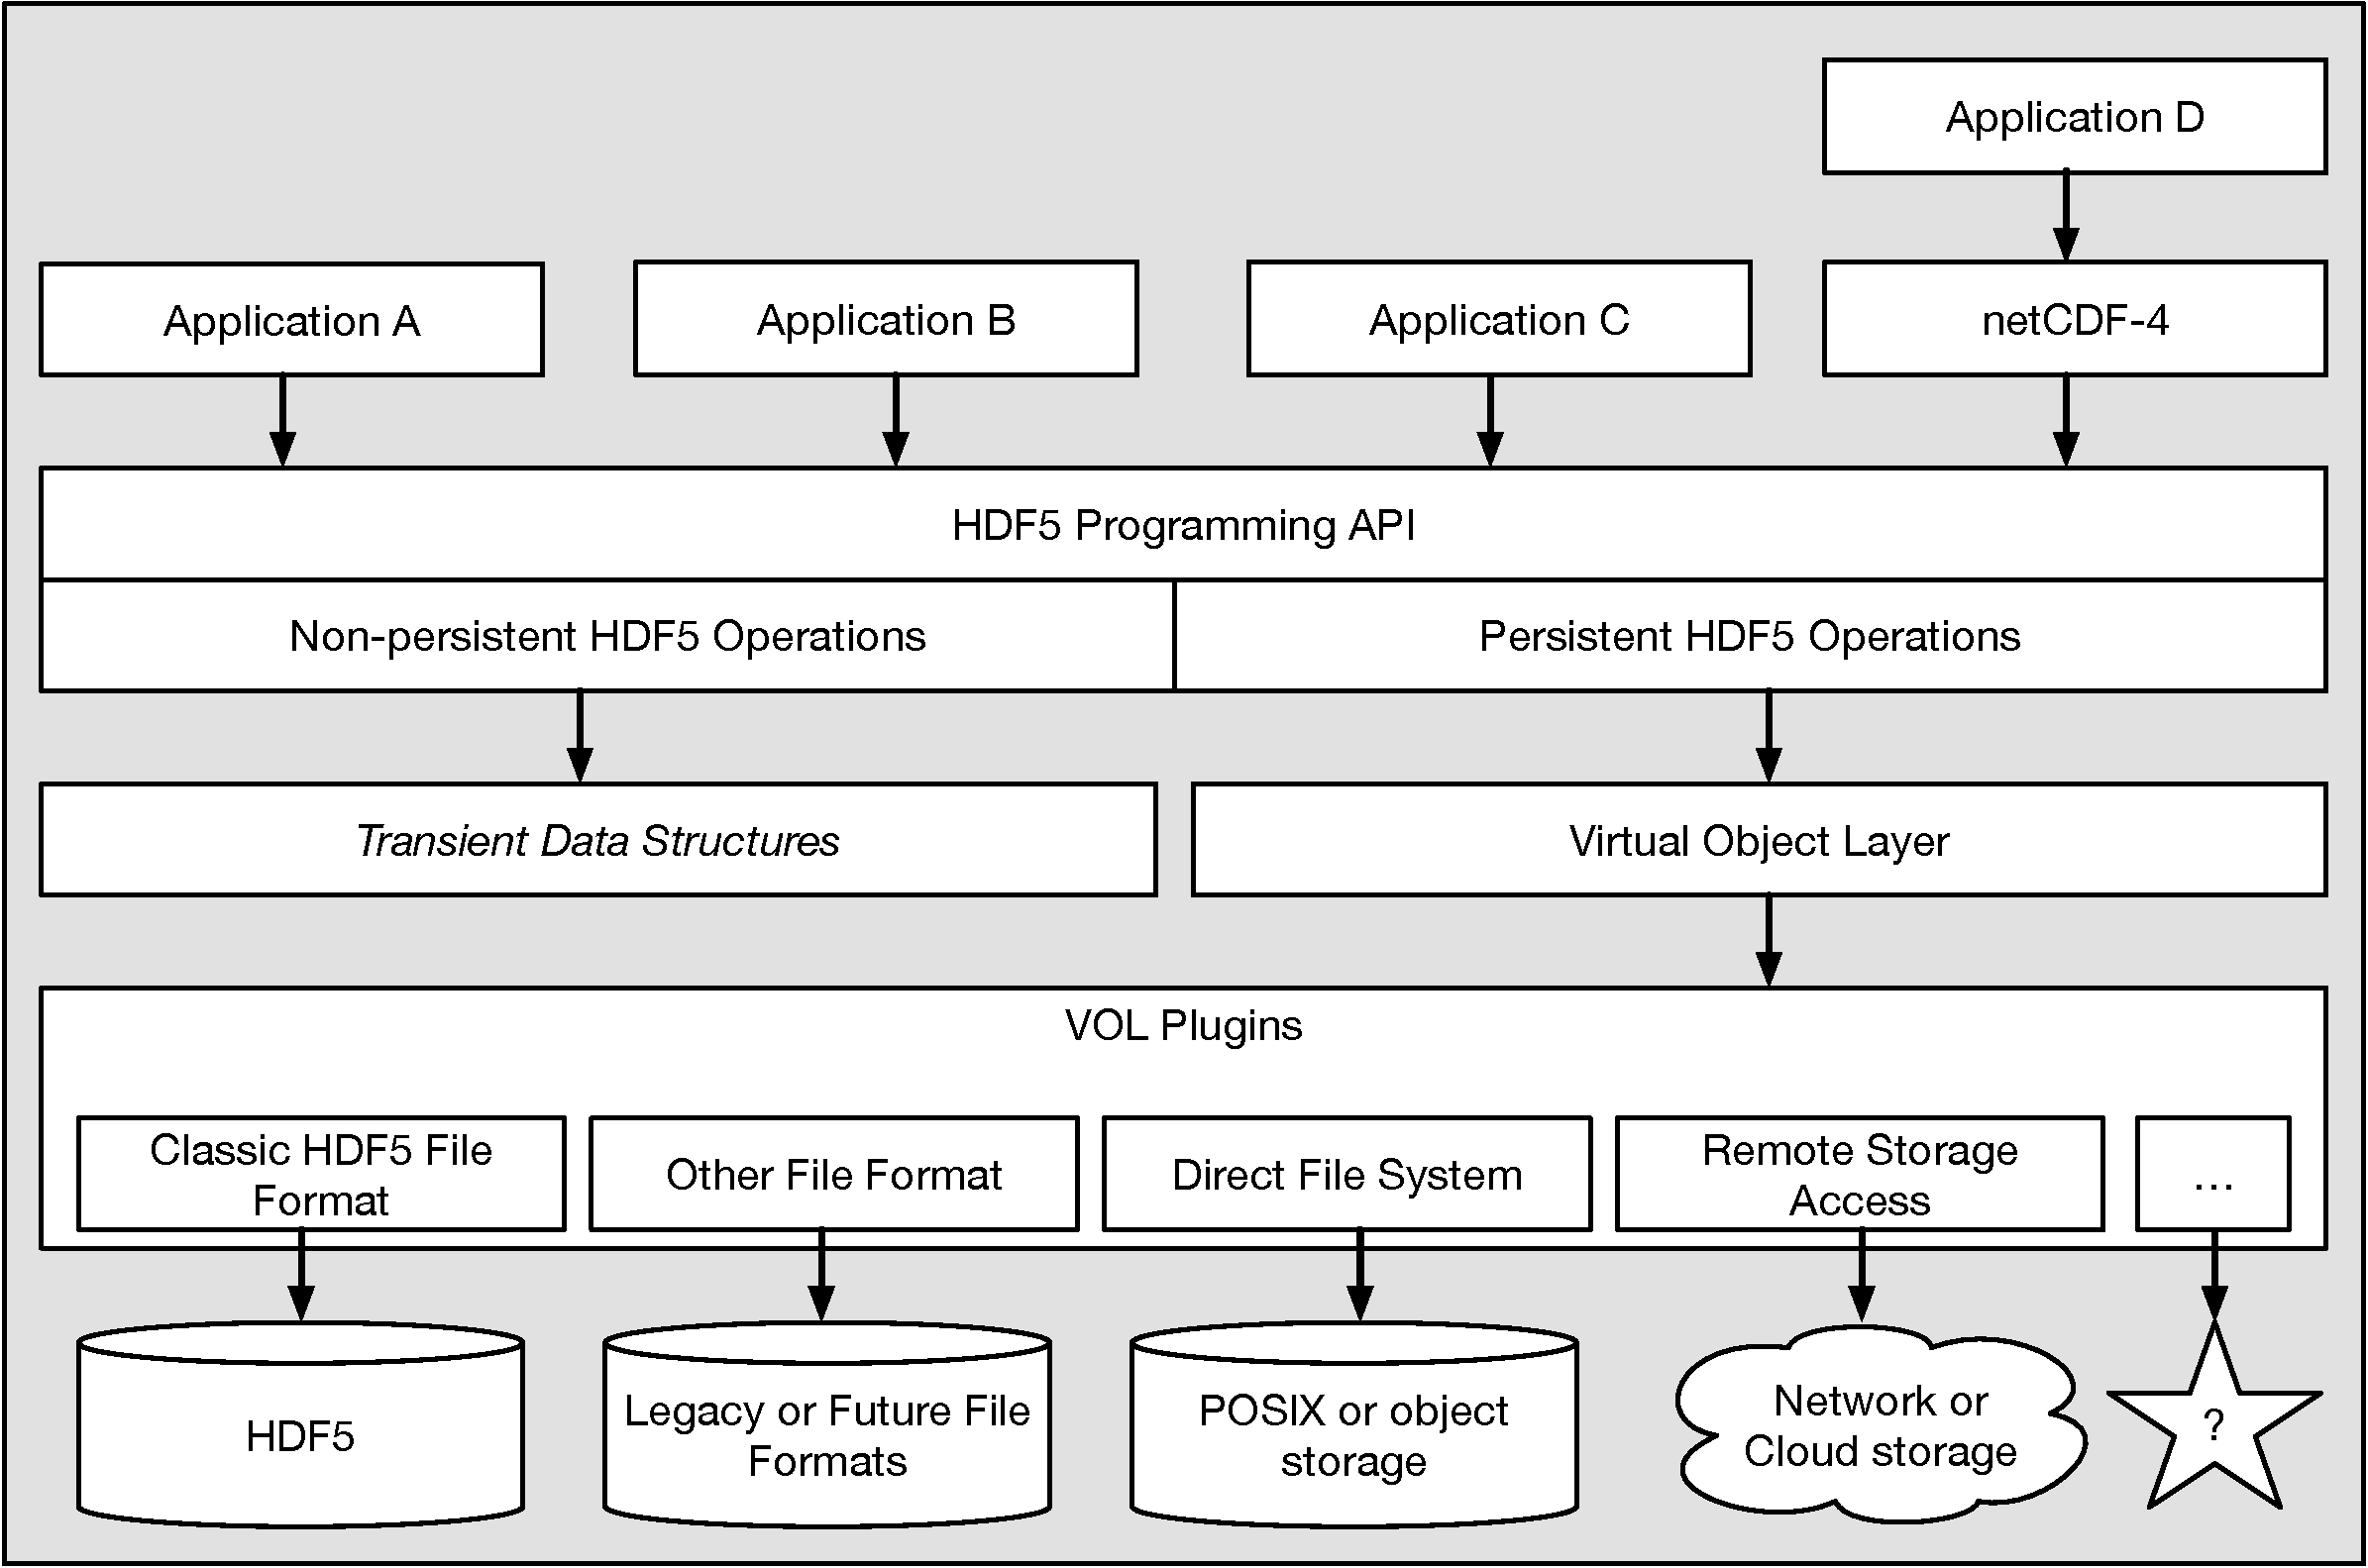
\includegraphics[width=0.48\textwidth]{projects/2.3.4-DataViz/2.3.4.08-ExaHDF5/VOL-Overview.pdf}
  \end{center}
  \caption{An overview of Virtual Object Layer (VOL)}
  \label{fig:vol-overview}
\end{wrapfigure}

\textit{Interoperability with other file formats.} To open the HDF5 API for interfacing with various file formats and to provide the capability of intercepting HDF5 API calls,  Virtual Object Layer (VOL) feature is being developed. the Virtual Object Layer (VOL) adds a new abstraction layer internally to the HDF5 library and is implemented just below the public API. The VOL intercepts all HDF5 API calls that access objects in a file and forwards those calls to an “object driver” plugin. A VOL plugin can store HDF5 data model objects in a variety of ways. Figure \ref{fig:vol-overview} shows a high-level view of VOL, where intercepted HDF5 API can interface with other file formats and object storage. We will create VOL plugins to access the netCDF and ADIOS/BP file formats, so that applications can use the HDF5 API to operate on data stored in these formats. The interoperability functions in the VOL support the pre-defined datatypes (integers, floating-point values, strings, etc.) in these formats, and will also support compound datatypes, i.e., a user-defined combination of pre-defined datatypes, in netCDF and will use compound datatypes to support ADIOS’ complex datatypes, which represent complex numbers.


\paragraph{Recent Progress}
\emph{Prototype implementation of Data Elevator read prefetching.} The project team has developed a prototype implementation of read caching and prefetching functionality and tested with various data read kernels from real applications. Using the burst buffers on Cori, the Data Elevator achieves 1.2 to 3X performance improvement over a highly tuned HDF5 code in reading data. Performance evaluation included representative I/O of convolution on climate modeling data, gradient computation of a plasma physics data, and voriticity computation of a combustion dataset. 

\emph{Integration of VOL into the develop branch. } VOL branch has been integrated into the main HDF5 development branch. Earlier in the project, an older VOL branch was brought in sync with the latest development branch. The development branch with the VOL feature has been tested with various VOL connector codes. A pass-through VOL connector also has been developed to test stack-ability of multiple VOL connectors. 

\emph{Supporting ECP application I/O}
The ExaHDF5 team has been working with various applications in the ECP portfolio. Applications and the AMReX co-design center have seen some performance issues, mainly because of less optimal configurations, such as using too few file system servers (e.g. Lustre Object Storage Targets or OSTs), producing a large number of metadata requests, using MPI collective buffering that was observing poor performance on NERSC's Cori. By simply changing these configurations, HDF5 achieved higher performance in writing files. 

\paragraph{Next Steps}

The ExaHDF5 team is developing indexing and querying feature, capability to read data in other file formats (ADIOS, netCDF), and topology-aware I/O, and asynchronous I/O. The Data Elevator read caching and prefetching function is being tested for release and deploy on the NERSC's Cori system. 

